\section{Ильясова Алина - Иностранные инвестиции}

Бюджет: 100.000 евро

Я решила одну половину денег вложить в экономики других стран через Московскую биржу посредством покупки ETF (вид ценных бумаг, выполняющих роль сертификата на портфель акций, облигаций, биржевых товаров), а другую половину вкладывать в акции компаний других стран посредством иностранного брокера.

subsection{ETF или ПИФы?}

Так как я не хочу тратить время на самостоятельный выбор акций и облигаций, я буду пользоваться готовыми инструментами коллективных инвестиций (ПИФы и ETF).

ETF (Exchange Traded Fund, биржевой инвестиционный фонд) – это инструмент коллективных инвестиций, созданный на базе фондовой инфраструктуры и допущенный к обращению на бирже для неограниченного круга лиц, имеющий эффективный механизм выпуска и погашения акций через уполномоченных лиц (авторизованных участников). Как правило, ETF отслеживает индекс акций или облигаций (например, MSCI Germany, Barclays Emerging Markets Tradable Russian Corporate Bond (EMRUS) Index) или металла (золота). Торгуется на Московской бирже и других мировых биржевых площадках как акция.

Сравним ПИФы и ETF:

\begin{center}
	\begin{tabular}{ccc}
	      & \textbf{ETF} & \textbf{ПИФы} \\
	      \textbf{Где купить} & На бирже & На бирже или в офисе \\
	       & & управляющей компании \\
	      \textbf{Комиссии} & В пределах 1\% & 3-8\% \\
	      \textbf{Ликвидность} & Высокая & Низкая \\
	      \textbf{Защита} & Российское+европейское & Российское законодательство \\
	       & законодательство & \\
	\end{tabular}
\end{center}

Я считаю, что ПИФы нужно в следующих случаях:
\begin{itemize}
	\item если человек не хочет открывать брокерский счет
	\item если человеку нельзя инвестировать в иностранные активы, которыми являются ETF (например, он госслужащий)
\end{itemize}

Сразу оговорюсь, что на Санкт-Петербургской бирже можно самостоятельно собрать пакет из иностранных акций, но я не хочу тратить на это время, поэтому буду открывать брокерский счет на Московской бирже.

Несомненным минусом ETF является то, что на Московской бирже всего 2 провайдера:
\begin{itemize}
	\item FinEx - 13 ETF
	\item ITI Funds - 2 ETF
\end{itemize}

Я буду рассматривать ETF, провайдером которых является FinEx.

\subsection{Составы различных ETF}

\subsubsection{Акции Китая (FXCN)}

Крупнейшие вложения:

\begin{itemize}
	\item TENCENT HOLDINGS LI (CN) - 14,23\%
	\item ALIBABA GROUP HLDG ADR - 11,66\%
	\item CHINA CONSTRUCTION BK H - 5,39\%
	\item CHINA MOBILE - 4\%
	\item BAIDU ADR - 3,4\%
	\item PING AN INSURANCE H - 3,38\%
	\item ICBC H - 3,25\%
	\item BANK OF CHINA H - 2,31\%
	\item CNOOC - 1,96\%
	\item CHINA PETRO \& CHEM H - 1,45\%
\end{itemize}

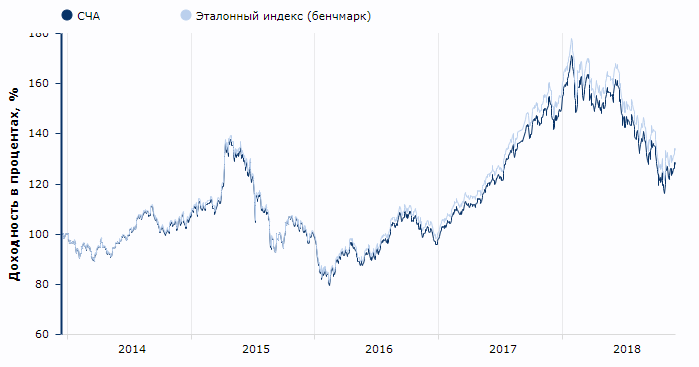
\includegraphics[width=16cm]{pics/alina/china.png}

\subsubsection{Акции США (FXUS)}

Крупнейшие вложения:

\begin{itemize}
	\item APPLE - 3,7\%
	\item MICROSOFT CORP - 3,21\%
	\item AMAZON.COM - 2,67\%
	\item JOHNSON \& JOHNSON - 1,62\%
	\item JPMORGAN CHASE \& CO - 1,56\%
	\item EXXON MOBIL CORP - 1,4\%
	\item ALPHABET C - 1,39\%
	\item FACEBOOK A - 1,38\%
	\item ALPHABET A - 1,33\%
	\item BERKSHIRE HATHAWAY B - 1,15\%
\end{itemize}

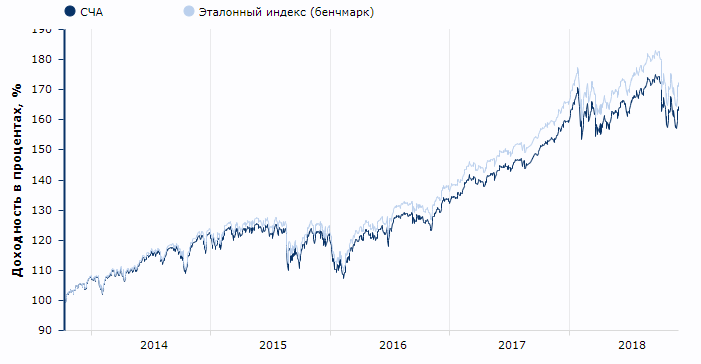
\includegraphics[width=16cm]{pics/alina/usa.png}

\subsubsection{Акции IT-компаний США (FXIT)}

Крупнейшие вложения:

\begin{itemize}
	\item APPLE	- 4,82%
	\item MICROSOFT CORP - 12,84%
	\item ALPHABET C - 5,56%
	\item FACEBOOK A - 5,51%
	\item ALPHABET A - 5,32%
	\item VISA A - 4,09%
	\item INTEL CORP - 3,74%
	\item CISCO SYSTEMS - 3,60%
	\item MASTERCARD A - 2,97%
	\item ORACLE CORP - 2,54%
\end{itemize}

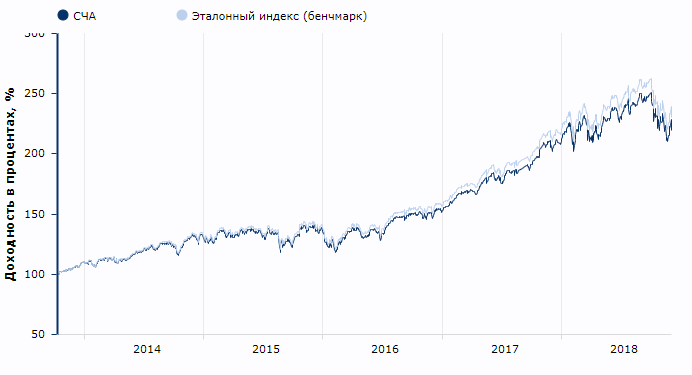
\includegraphics[width=16cm]{pics/alina/usait.png}

\subsubsection{Акции Германии (FXDE)}

Крупнейшие вложения:

\begin{itemize}
	\item SAP - 8,51\%
	\item ALLIANZ - 7.93\%
	\item SIEMENS - 7,47\%
	\item BASF - 5,96\%
	\item BAYER - 5,66\%
	\item DEUTSCHE TELEKOM - 4,95\%
	\item DAIMLER - 4,48\%
	\item ADIDAS - 3,73\%
	\item MUENCHENER RUECKVERSICH -2,79\%
	\item VOLKSWAGEN VORZUG - 2,74\%
\end{itemize}

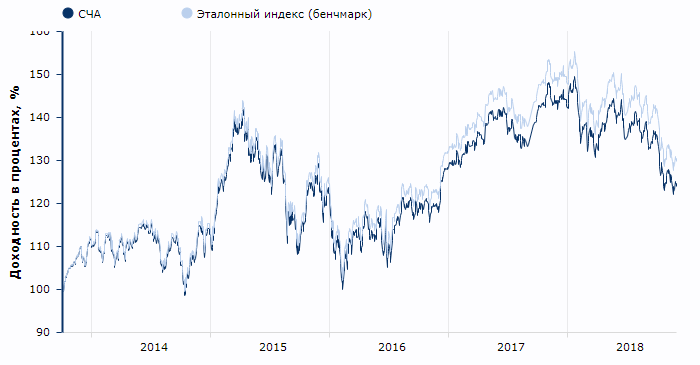
\includegraphics[width=16cm]{pics/alina/germany.png}

\subsubsection{Акции Японии (FXJP)}

Крупнейшие вложения:

\begin{itemize}
	\item TOYOTA MOTOR CORP - 4,28\%
	\item MITSUBISHI UFJ FIN GRP - 2,09\%
	\item SOFTBANK GROUP CORP - 2,03\%
	\item SONY CORP - 2,03\%
	\item KEYENCE CORP - 1,57\%
	\item SUMITOMO MITSUI FINL GRP - 1,54\%
	\item HONDA MOTOR CO - 1,44\%
	\item KDDI - 1,27\%
	\item MIZUHO FINANCIAL GROUP - 1,27\%
	\item MITSUBISHI CORP - 1,14\%
\end{itemize}

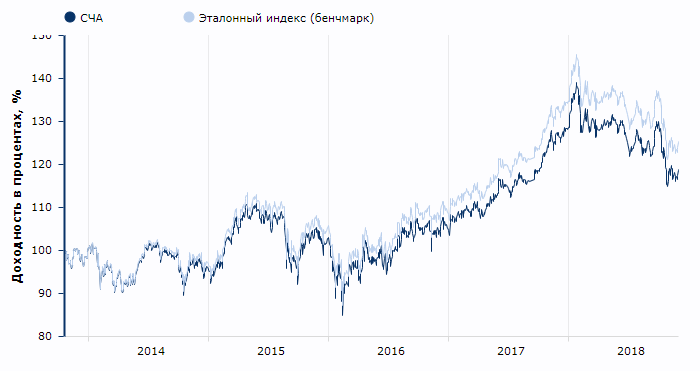
\includegraphics[width=16cm]{pics/alina/japan.png}

\subsubsection{Акции Австралии (FXAU)}

Крупнейшие вложения:

\begin{itemize}
	\item COMMONWEALTH BANK OF AUS - 10,20\%
	\item BHP BILLITON (AU) - 8,40\%
	\item WESTPAC BANKING - 7,25\%
	\item CSL - 6,69\%
	\item ANZ BANKING GROUP - 6,09\%
	\item NATIONAL AUSTRALIA BANK - 5,41\%
	\item WOOLWORTHS GROUP - 3,14\%
	\item MACQUARIE GROUP -3,02\%
	\item WESFARMERS - 3,00\%
	\item TRANSURBAN GROUP - 2,46\%
\end{itemize}

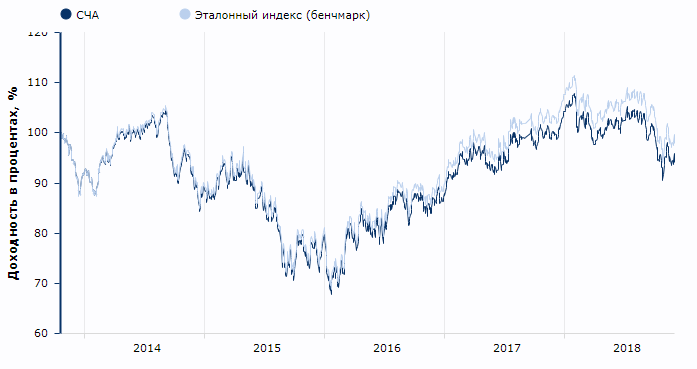
\includegraphics[width=16cm]{pics/alina/australia.png}

\subsubsection{Акции Англии (FXUK)}

Крупнейшие вложения:

\begin{itemize}
	\item HSBC HOLDINGS (GB) - 7,35\%
	\item ROYAL DUTCH SHELL A - 6,15\%
	\item BP - 5,88\%
	\item ROYAL DUTCH SHELL B - 5,10\%
	\item ASTRAZENECA - 4,36\%
	\item GLAXOSMITHKLINE - 4,34\%
	\item DIAGEO - 3,86\%
	\item BRITISH AMERICAN TOBACCO - 3,47\%
	\item UNILEVER PLC (GB) - 2,90\%
	\item RIO TINTO PLC (GB) - 2,54\%
\end{itemize}

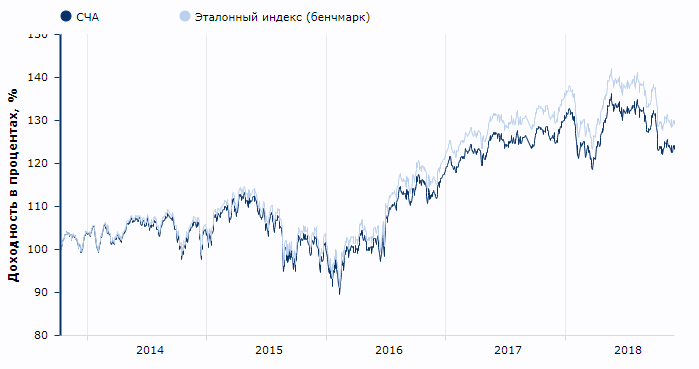
\includegraphics[width=16cm]{pics/alina/uk.png}

\subsubsection{Акции Казахстана (FXKZ)}

Крупнейшие вложения:

\begin{itemize}
	\item KAZ MINERALS PLC GBP0.2 - 16,09%
	\item KAZAKHTELECOM KZT1000 - 15,18%
	\item KAZAKHSTAN ELECTRICITY GRID NPV - 14,86%
	\item KCELL JSC NPV - 14,67%
	\item KAZTRANSOIL JSC NPV - 14,61%
	\item HALYK SAVINGS BANK-KAZAKHSTN NPV - 14,53%
	\item BANK CENTERCREDIT NPV - 10,06%
\end{itemize}

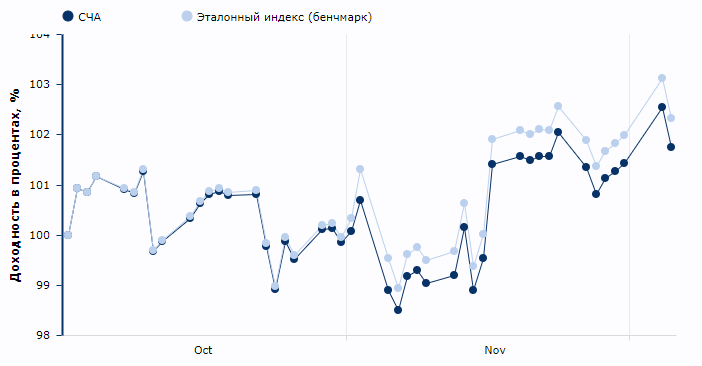
\includegraphics[width=16cm]{pics/alina/kz.png}

\subsubsection{Другие ETF:}

\begin{itemize}
	\item FXMM - гособлигации США
	\item FXGD - акции на золото
	\item FXRB и FXRU - еврооблигации самых надежных российских эмитентов
	\item FXRL - акции индекса Московской Биржи
\end{itemize}

\subsection{Конвертация денег}

Сначала мы проведем конвертацию евро в рубли, а потом рубли в евро. Для экономии времени будем делать это в одном банке.

6 февраля 2018 года лучший курс из топ-10 банков России (по рейтингу интернет-портала banki.ru) был у Альфа-банка с курсом евро (продажа) = 76,2 и курсом доллара (покупка) = 66,3

Таким образом, 100.000 евро = 114.932 доллара США.

\subsection{Выбор брокера}

Восемь ETF из двенадцати на Московской бирже можно купить как за рубли, так и за доллары США через брокеров:

\begin{itemize}
	\item ВТБ
	\item ЦЕРИХ
	\item КИТ Финанс
	\item УРАЛСИБ
	\item Райффайзенбанк
\end{itemize}

\subsubsection{ВТБ}

Тарифы:

\textbf{Тариф «Инвестор стандарт»}

Комиссия Банка *, ** — 0,0413%

\textbf{Тариф «Профессиональный стандарт»}

Комиссия Банка *, ** —

-при дневном обороте до 1 млн. руб. включительно — 0,0472%

-при дневном обороте от 1 до 5 млн. руб. вкл.— 0,0295%

-при дневном обороте от 5 до 10 млн. руб. вкл.— 0,02596%

-при дневном обороте от 10 до 50 млн. руб. вкл.— 0,02124%

-при дневном обороте от 50 до 100 млн. руб. вкл.— 0,0195%

-при дневном обороте свыше 100 млн. руб. — 0,015%

* НДС не облагается.

Под суммой оборота понимается оборот по сделкам с ценными бумагами** и сделкам купли-продажи иностранной валюты, заключенным после 19:00 предыдущего торгового дня до 19:00 текущего торгового дня.

**  за исключением сделок в Торговых системах с облигациями федерального займа для физических лиц (ОФЗ-н) и сделок в ТС Основной рынок ФБ ММВБ с ценными бумагами, по которым установлен срок обращения от 1 до 7 дней (включительно).

\subsubsection{ЦЕРИХ}

Тарифы:

\textbf{Отличный старт.} Удобный тариф для начинающих инвесторов. Регулярная аналитическая поддержка. Торговые рекомендации от наших аналитиков позволят чаще совершать прибыльные сделки, а аналитическая справка к каждой идее - учиться, на что обращать внимание при изучении рынков

Комиссия: 0,2\% от суммы сделки

\textbf{Инвестор.} Тариф оптимален для клиентов, использующих средне- и долгосрочные портфельные инвестиции. Величина комиссионного сбора определяется в зависимости от суммы чистых активов на счете – чем больше средств, тем меньше вознаграждение.

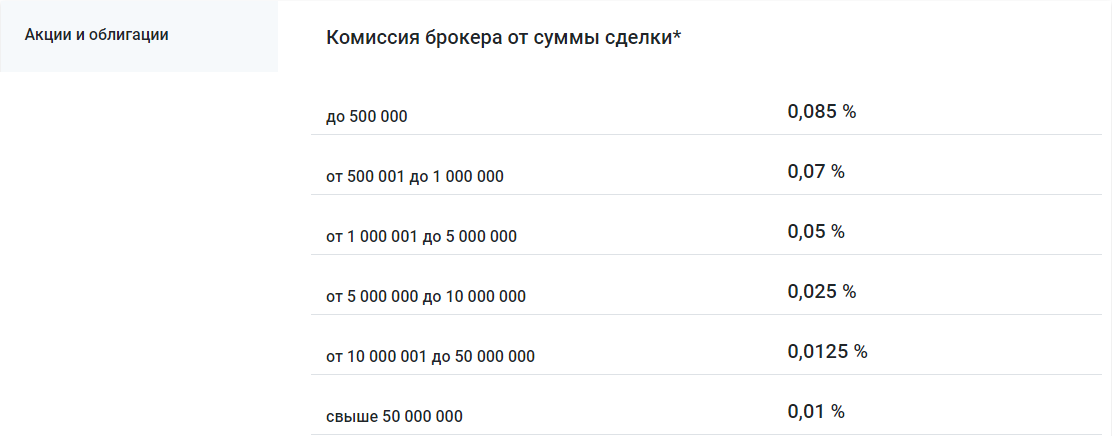
\includegraphics[width=16cm]{pics/alina/cerih_invest.png}

\subsubsection{КИТ Финанс}

Тарифы:

\textbf{КИТ-Стандарт}

Комиссия за сделку (в зависимости от оборота в день):

-До 1 млн.руб. - 0,048\%

-От 1 до 7,5 млн.руб. - 0,032\%

-Свыше 7,5 млн.руб. - 0,025\%

\textbf{КИТ-Команда}

Коммисия за сделку: 0,1\%

\textbf{КИТ-Инвестор}

Комиссия за сделку (в зависимости от оборота в день):

-До 300 тыс.руб. - 0,5\%

-От 300 тыс. до 1 млн.руб. – 0,35\%

-Свыше 1 млн.руб. – 0,1\%

\textbf{КИТ-Сделка}

Коммисия за сделку: 1,5\%, минимум 2800 рублей за поручение

\subsubsection{УРАЛСИБ}

Тарифы:

\textbf{Тарифный план №1 «Основной»}

Комиссия брокера,\% от торгового оборота за месяц:

- до 10 000 000 - 0,0472

- от 10 000 000 до 30 000 000 - 0,0413

- от 30 000 000 до 50 000 000 - 0,0377

- от 50 000 000 до 100 000 000 - 0,0330

- от 100 000 000 - 0,0236

\textbf{Тарифный план №2 «Дневной»}

Комиссия брокера,\% от торгового оборота за день:

- до 500 000 - 0,0472

- от 500 000 до 1 500 000 - 0,0354

- от 1 500 000 до 5 000 000 - 0,0295

- от 5 000 000 до 10 000 000 - 0,0236

- от 10 000 000 - 0,0212

\subsubsection{Райффайзенбанк}

Категории обслуживаемых клиентов:

На сегодняшний день для физических лиц брокерское обслуживание предлагается клиентам банка — держателям пакета услуг банка «Премиальный 5» и «Премиальный».

Рекомендуемая сумма инвестиций:

- Биржевой рынок: от 1 млн рублей / 15 тысяч долларов США.

- Внебиржевой рынок: от 200 тысяч долларов США.

\subsubsection{В итоге:}

Я решила выбрать ВТБ-24, так как у них самый адекватный уровень соотношения надежность-размер комиссии.

\subsection{Выбранные ETF}

В долларах можно вкладываться только в следующие ETF, состоящие из иностранных акций:

\begin{itemize}
	\item FXAU
	\item FXCN
	\item FXJP
	\item FXUS
	\item FXIT
	\item FXGD
\end{itemize}

В каждый из этих ETF я буду вкладывать по \textbf{19.155\$}.

\subsubsection{FXAU}

Стоимость одной акции - 26.98\$

Доходность индекса за 5 лет - 3,86\%

В итоге денег = 19.705

\subsubsection{FXCN}

Стоимость одной акции - 38.42\$

Доходность индекса за 5 лет - 29\%

В итоге денег = 24.475

\subsubsection{FXJP}

Стоимость одной акции - 35.14\$

Доходность индекса за 5 лет - 25,61\%

В итоге денег = 23.832

\subsubsection{FXUS}

Стоимость одной акции - 47.71\$

Доходность индекса за 5 лет - 63.40\%

В итоге денег = 31.001

\subsubsection{FXIT}

Стоимость одной акции - 65.19\$

Доходность индекса за 5 лет - 120,98\%

В итоге денег = 41.926

\subsubsection{FXGD}

Стоимость одной акции - 30,10\$

Доходность индекса за 5 лет - 17,8\%

В итоге денег = 22.350


\textbf{Общая сумма = 163.289}

\subsection{Риски инвестирования}

\begin{itemize}
	\item По-настоящему существенный риск в ETF ­­— это рыночный риск, обусловленный изменениями котировок ценных бумаг, процентных ставок, курсов валют. Это означает, что ETF всегда идет туда, куда идет рынок — цена акций растет, если растет индекс рынка, и падает, если фондовый индекс снижается. Полезно думать про биржевые индексные фонды ETF так – это лишь «прозрачная обертка» для инвестиций. Все остальные риски минимизированы за счет «устройства» ETF. В отличие от самостоятельного инвестирования или вложений в ПИФ, в ETF нет риска ошибки управляющего, по сравнению со структурным продуктом (нотой) — отсутствует риск банкротства эмитента, по сравнению с банком — минимум регулятивных рисков. Для тех, кто инвестирует в долгосрочной перспективе, рыночный риск не является  проблемой. Диверсифицированный портфель из ETF на горизонте инвестиций в десять и более имеет свойство отыгрывать даже значительные падения – инвестор на выходе получает ожидаемую прибыль.
	\item Также существует риск банкротства брокера. Зачастую в контрактах прописан пункт, что брокер может одалживать у клиента ценные бумаги, при исключении этого пункта из контракта, комиссии увеличиваются
\end{itemize}

\newpage

\section{Инфляция}

Уровень инфляции по годам в Еврозоне, \%:

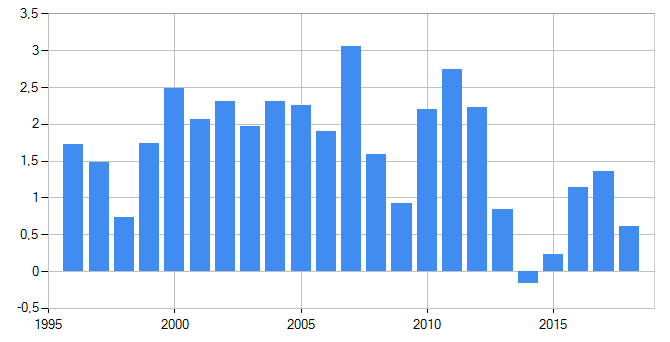
\includegraphics[width=16cm]{pics/alina/inflation.png}

Рассмотрим 3 варианта событий:

\begin{itemize}
	\item Низкий уровень - 0,7\%. Через 5 лет с учетом инфляции 700.000 евро будут эквивалентны 725.845 евро
	\item Средний уровень - 1,7\%. Через 5 лет с учетом инфляции 700.000 евро будут эквивалентны 761.558 евро.
	\item Высокий уровень - 3,1\%. Через 5 лет с учетом инфляции 700.000 евро будут эквивалентны 815.439 евро
\end{itemize}